\documentclass[12pt]{article}
\usepackage[utf8]{inputenc}
\usepackage{fancyhdr}
\usepackage{graphicx}
\usepackage{geometry}
\usepackage{float}
\usepackage[utf8]{inputenc}
\usepackage{authblk}
 
\usepackage{array}
\usepackage{makecell}

% ---- Commands ------- %
\newcommand{\documentNumber}[1]{
    \LARGE  \textbf{Slutrapport}
    \\
    \medskip
}
\graphicspath{ {./images/} }
\newcommand{\documentVersion}[1]{
    \medskip
}
\newcommand{\documentTitle}[1]{
    \centerline{\rule{13cm}{0.4pt}}
    \bigskip \bigskip
    \LARGE \textbf{MAMF40} \\
    \bigskip
    \LARGE {#1} \\
    \bigskip \bigskip
    \centerline{\rule{13cm}{0.4pt}}
}

\newcommand{\documentDate}[1]{
    \date {#1} 
}

\renewcommand\theadalign{bc}
\renewcommand\theadfont{\bfseries}
\renewcommand\theadgape{\Gape[5pt]}
\renewcommand\cellgape{\Gape[5pt]}


\renewcommand{\contentsname}{Innehållsförtäckning}

% --- Header & Footer ---- %
\pagestyle{fancy}
\lhead{\leftmark}
\rhead{}
\rfoot{\thepage}
\cfoot{}
\lfoot{}


% ------------------------------------------------ #

% ----- FILL THIS ----- %
\title {
    \documentNumber {01}    

    % Full name - SHORTNAME
    \documentTitle {Helsingborg Event and Convention Bureau}
    
    % Format: YYYY-MM-DD
    \documentDate {\today}
    \documentVersion Vv 1.0
    
\author{Anna Bergvall - Oscar Blixt - Pontus Persson\\\\ David Vilppu - Filip Sjövall - Sabah Zafar}



}

%\author{
%  Anna Bergvall\\
%  \and
 % Filip Sjövall\\
%   \and
 % David Vilppu\\
 %   \and
 % Oscar Blixt\\
%    \and

% Sabah Zafar\\
 %   \and
 % Pontus Persson\\
%}






\begin{document}
\addtocontents{toc}{\protect\setcounter{tocdepth}{2}}
\maketitle
%%\end{document}
\thispagestyle{empty}



\newpage

\tableofcontents



\newpage

%\ dokument historia ska inte vara med
%section{Dokument Historia}
%\begin{tabular}{ l | l | l }
 %   Version & Datum & Beskrivning \\
  %  \hline
 %   0.1 & 2021-09-29 & Dokumentet skapat. \\
 %    \hline
   
   
%\end{tabular}


\newpage
% ----- SKRIV UNDER VARJE TITEL ----- %

\section{Arbetsfördelning}
\textbf{Filip}: Haft rollen som projektledare vilket har medfört arbete som att planerat sprintar, förvalta scrumboarden och vara talesperson vid interna och externa möten. Utöver rollen som projektledare har Filip jobbat med allt inom hemsidan och dokument, från att skapa templates med html och css för frontend till att implementera funktioner på hemsidan med API och javascript och tillslut skriva i slutrapporten.\\\\
\textbf{Anna}: Varit projektledare tillsammans med Filip. Detta har lett till en delad arbetsfördelning med att förvalta scrumboarden och planera sprintar. Har också haft ansvar för mail med kunden. Vid möten har Anna tagit rollen som sekreterare, Anna har generellt jobbat mycket med dokument tillexempel slutrapporten. Utöver detta har hon fokuserat på arbete med databas och API för att implementera funktioner som inloggning för admin  och varit med och skrivit databasen.\\\\
\textbf{David}: Arbetat med lite av allt inom projektet. Till en början hade David större delaktigthet i att designa databasen men gick senare över till att hjälpa till med design, som att designa utseende på knappar och att implementera funktioner i backend. I slutet av projektet hade David hand om användartesing samt att skriva i slutrapporten.\\\\
\textbf{Oscar}: Har genom hela projektet haft stort fokus på arbete med databas och api. Att implementera allt från inlogging för admin och svarspersoner, sammaställa data för brancher samt att skriva stora delar av databasen. Oscar har även varit lite delaktigt i att skriva slutrapporten.\\\\
\textbf{Sabah}: Genom projketet har Sabah haft ansvar för dokument som Processrapport och arbetsrapport. Under projketet har Sabah dokumenterat det gruppen har gjort via arbetsrapporten och kontinuerligt skrivit i slutrapporten. Senare under projektet har Sabah också arbetat med testfall.\\\\
\textbf{Pontus}: Har tagit stort ansvar för api:n under projektet. Från att undersöka vilka programmeringsvertyg gruppen skulle använda för att tackla uppgiften, till att implementera stora moment som att få formuläret att gå mellan olika frågor, spara användardata i cookies samt skicka denna data till databasen. I slutet av projektet har Pontus även tagit ansvar för hur  systemet skall diftsättas på en server.\\\\
\section{Abstract}
Sustainability is becoming an increasingly important part of businesses’ and organisation’s values. As a result, a wide array of sustainability certificates are attainable for showing environmental good-will and to support continuous efforts. One of these certificates is Global Destination Sustainability Movement (GDSM). The city of Helsingborg, a national hub for events and conferences, is aiming to acquire this certificate. In order to be a part of GDSM, cities must fill in a form containing 69 criteria ”that measures, benchmarks and improves the sustainability strategy and performance of tourism and events destinations” (GDS-Index 2021, Methodology).\\\\
For the purpose of collecting sustainability data from hotels and restaurants in Helsingborgs stad, a web based questionnaire was developed. The data was saved in a database using MySQL through the Flask API, written in Python. To ensure a mobile friendly and responsive application, the system was built using the CSS framework Bootstrap. 
Given the fact that the success of the project was dependent on response frequency, making the system easy to use for users of various technichal backgrounds was paramount. 

(and then something about user testing maybe)

\newpage
\section{Introduktion}
Vår kund Helsingborg Convention and Event Bureau(HCEB)\footnote{https://helsingborgceb.com/} önskade att gå med i det globala nätverket Global Destination Sustainability Movement (GDSM). Som medlem i nätverket rapporteras det årligen in hållbarhetsdata som bidrar till en positiv utveckling av staden som en mötes- och evenemangsdestination. Målet med projektet är att utveckla ett digitalt rapporteringsverktyg som samlar in och sammanställer hållbarhetsdata från aktörer inom besöksnäring i städer och kommuner. Rapporteringsverktyget erbjuder en skräddarsydd sammanställning och större kontroll över distribution och administration av den insamlade datan. Det utvecklade rapporteringsverktyget är en webbaserad hemsida som ska användas av aktörer med olika tekniska färdigheter, vilket gör att stora krav ställs på användarvänlighet.







\section{Process}

\subsection{Planering}
En fördel med ett agilt arbetssätt där det finns en tät kontakt med uppdragsgivare är att det upprätthåller en regelbunden kommunikation mellan kunden och utvecklingsteamet där fungerande programvara prioriteras över utförlig dokumentation. Dessutom värderas möjlighet för anpassning och förändring. Projektgruppen har därför valt att tillämpa Scrum [1].  \\\\
Projektets mål var att utveckla ett fungerande rapporteringsverktyg som ska användas av Helsingborg Convention and Event Bureau för sammanställning av \\ hållbarhetsdata från aktörer verksamma inom besöksnäringen i Helsingborg. \\\\
Utifrån målbildanalysen valdes en lättrörlig projektmodell eftersom informationen och kunskapen om projektet i det inledande skedet var knapp. Gruppen ville snabbt kunna agera och ta beslut om arbetet skulle gå i fel riktning vilket det kan finnas risk för i början. Medlemmarna ville på det sättet ha frihet att kunna ta beslut i efterhand om det exempelvis skulle dyka upp nya krav. Förhoppningen var att detta skulle leda till en mer flexibel och anpassningsbar utveckling. Av denna anledning beslutades det att inledningsvis sätta våra sprints till en vecka. \\\\ 
En annan anledning till att arbeta med en lättrörlig modell var möjligheten att hela tiden jobba med en testbar produkt istället för att bara arbeta med en slutprodukt. Med andra ord var målet att jobba med "evolutionary prototypes" som inte skulle kasseras mellan varje användartest utan snarare vidareutvecklas enligt kundens önskemål [1].\\\\
Senare i projektet arbetades enligt en iterativ process eftersom en tydligare målbild hade skapats och gruppen kunde strukturera upp arbetet utifrån detta. Efter struktureringen valde gruppen att jobba utifrån en scrumboard där den uppgift som fanns högst upp på scrum boarden skulle bli tagen först. \\\\
För att säkerställa att alla gruppmedlemmar var uppdaterade med rätt information hade vi kommunikation på discord. På schemat fanns även många inplanerade interna möten för att kunna ta viktiga besult och diskutera utvecklingsarbetet. Kunden var också involverad i arbetet genom en kontinuerligt kontakt vid förutbestämda möten med jämna mellanrum. Dessutom skapades en gemensam mailadress inom projektgruppen för mailkommunikation med kunden under utvecklingen.\\\\
%- Test av HiFo prototyp - flytta ett en annan sektion men diskutera under Diskussion 
\subsection{Användbarhetstestning}
För att utvärdera den slutliga prototypen skapades några testscenarier med frågor som rör användbarhet och användarupplevelse. Observationstest planerades på ett sätt där en  testperson skulle interagera med prototypen av webbplatsen baserat på testscenarierna utan att förklara sitt agerande och utan ett ingripande av observeraren. Det för att låta testpersonen göra val baserat på deras naturliga användning av hur de i verkligheten skulle svara på frågeformuläret på vår utvecklade rapporteringsverktyg. Dessa interaktioner skulle sedan dokumenteras och  analyseras.\\\\
Under en testsession fick testpersonen uppgiften att utföra olika moment som till exempel: "Logga in med användarnamn X", "Svara på formuläret." och "Lägg till en ny användare.". Med hjälp av testerna kunde projektmedlemmarna notera eventuella moment eller funktioner som inte uppfyllde gruppens krav på intuitet och därmed korrigera dessa. Om inga brister i användbarheten hittades gav testerna en möjlighet att bekräfta uppfyllandet av användbarhetskrav.\\\\
Användbarhetstesterna gjordes av totalt 4 försökspersoner vars bakgrund var variende både gällande ålder och datorkunskaper. En del av försökspersonerna jobbade dagligen med datorer medan andra hade måttlig interaktion med en dator och var flitiga användare av mobiltelefonen. \\\\
Försökspersoner valdes med baktanken om att de skulle vara av varierande karaktär för att mer rättvist spegla vår slutanvändare. Efter en testsession ställdes öppna frågor som till exempelvis "Var det något du tänkte på under tiden du svarade på frågorna?", varpå deras svar noterades och analyserades tillsammans med samtliga gruppmedlemmar.\\\\
Användbarhetstesterna var grunden för att kunna ändra systemets innehåll i syfte att göra systemet mer uppenbart och intuitivt för användaren.


\subsection{Utveckling}
\textbf{Sprint ett, vecka 40}
Under första sprinten skulle ER-digaram samt flödesdiagram skulle framställas. Gruppen beslutade sig om att slopa UML-diagram utifrån inspiration från Matz, K [3] där det läggs fram att det vid agil utveckling behövs mindre dokument. 
Intern inom gruppen bestämdes också att sprintens längd skulle minskas från två veckor till en vecka. Tanken var att minska den totala tiden det skulle ta att planera sprintar eftersom projektledarna kände att det var svårt att veta i förväg vad som skulle hända de kommande veckorna. Vid singel veckors sprintar kunde en mer adaptiv planering införas vilket passar tidigt i projektet eftersom det var en större osäkerhet på hur mycket arbete som behövde göras tidigt i projektet. \\\\
\\\\\textbf{Sprint två, vecka 43}\\\\
Efter \textbf{sprint ett} las arbetete med projektet på is på grund av tentaperioder, detta innebar också att inga beslut togs samtidigt som projektet stod stilla.
\textbf{Sprint tre, vecka 44}\\\\
Tack vare att tidsplaneringen inte innehöll någon tentavecka för uppehåll så hamnade projektgruppen efter i tidsplaneringen. Detta i sig ledde till att vi slutade jobba utifrån sprintar och istället arbetade flytande med att uppgifter som fanns i scrumboarden. Detta blev en naturlig övergång med tanke på att den tid som egentligen var utsatt för planering av sprintar istället gick åt till att koda. \\\\
\textbf{Sprint tre, vecka 45} \\\\
Det hade tidigare diskuterats om hur användaren skulle verifiera sig för att kunna svara på formuläret. Efter möte med kunden lades förslaget fram att användarna skulle identifiera sig med ett mailadress, detta istället för en specifik identifieringskod vilket tidigare hade varit förslaget. Detta för att göra det så enkelt som möjligt för både HCEB och användarna som skulle skicka in hållbarhetsdata.\\
Efter samtal med kunden beslutades det att arbetet skulle skalas av, istället för att skickat ut formuläret till samtliga aktörer skulle flygplatser och universitet uteslutas, detta för att det var så pass få aktörer inom dessa branscher.
\\\\
\textbf{Sprint tre, vecka 46} \\\
Utvecklingsarbetet tog fart och funktionalitet för adminsidan, admin login och logout, vidareutvecklades. Denna sprinten beslutades det att cookies skulle användas för att lagra användarens svar på samtliga frågor.\\\\
Ett annat beslut som togs under denna sprinten var att flytta scrumboarden från Atlassian till Trello, som hjälp i våra kommande sprintar. Atlassian var krånglig att använda, den hängde sig mycket och det var mer krävande att göra ändringar på Atlassian. Motiveringen att göra övergången var att scrumboarden skulle ses som ett hjälpmedel och inte ett hinder [2].\\\\
\textbf{Sprint fyra, vecka 47} \\\
Under denna sprinten började arbetet för att kunna mobilanpassa produkten och funktionaliteten för att kunna skicka in användarens svar till databasen implementerades.\\\\
Under sprinten togs beslut om att användaren skulle endast ha möjlighet att välja bland flervalsfrågor i form av knappar vilket skiljde sig från det tidigare sättet som möjliggjorde svarsalternativ i olika former. Ändringen ledde till att svarspersonen behövde göra mindre knapptryck för att gå vidare i formuläret vilket ledde till enklare inrapportering av data. Beslutet stöds också av [3] som menar att man endast ska visa nödvändig information för användarna samt att användaren ska kunna utföra ett uppgift med så lite tankekraft som möjligt.\\\\
\textbf{Sprint fem, vecka 48} \\\
Under denna sprinten fortsatte det tidigare påbörjade utvecklingen för systemet och inga ny beslut togs. \\\\
\textbf{Sprint sex, vecka 49} \\\
Utvecklingen fortsatte och tidigt under veckan färdigställdes all funktionalitet på hemsidan. Alla krav om funktioner som kunden hade i uppgifts-beskrivningen uppfylls.
\subsection{Riskanalys}
\subsubsection{Initial riskanalys}

 Tidigt i projektet, med hjälp av artikeln \textit{Riskanalys} [4], implementerades miniriskmetoden för att kunna identifiera riskerna och därefter analysera dem. En uppskattning av sannolikheten att dessa risker inträffar och konsekvenserna till följd av detta gjordes.\\\\
 Syftet med riskanalysen var att ta fram en åtgärdsplan som skulle följas vid hantering av risker, både proaktivt men även då eventuella risker är ett faktum. I riskanalysen skapades en lista över \textit{projektrisker, produktrisker} och \textit{affärsrisker}.\\\\
 Den största projektrisken som identifierades var en bristfällig kommunikation bland projektmedlemmarna. För att minimera denna risk skapades en tydlig kommunikationsplan samt grundregler. Denna åtgärd skulle leda till en bättre stämning i gruppen genom att missförstånd minimeras.\\\\
 Den största produktrisken som identifierades var att produkten inte skulle vara tillräckligt intuitiv, dvs. att användbarheten skulle bli för låg. För att minimera denna risk beslutades att utföra många användartester. Gruppen ansåg att detta skulle ge en god insikt om hur användare upplever systemet. \subsubsection{Plan för att uppdatera riskanalysen}
 Projektgruppen beslutade att i början av varje sprint koppla riskerna till de delmoment som sprinten innehöll för att kunna identifiera eventuella risker i den specifika sprinten. Om en gruppmedlem stötte på risker skulle detta meddelas under veckovisa möten, där riskerna kunde ställas mot åtgärdsplanen för att kunna hantera dessa omgående.
 \subsubsection{Genomförda ändringar i riskanalysen}Efter hand som vi arbetade med projektet blev det tydligt vilka risker som var relevanta och vilka som inte var ett så stort problem som vi hade tänkt oss i början. Att den största produktrisken var att produkten inte skulle vara tillräckligt intuitiv insåg vi snabbt inte stämde då vi upplevde det relativt enkelt att göra ett tillräckligt intuitivt frågeformulär.\\\\
 Däremot blev det tydligt att våra begränsade kunskaper kring servrar och databaser löpte än större risk att påverka projektets slutresultat. Därav såg vi just implementeringen av databas samt hemsida på en extern server som den största produktrisken.\\\\
 Gällande projektriskerna gjordes det inte några större ändringar. Kommunikationen är alltid svår, speciellt i en tid med pandemi och restriktioner. Vi gjorde vårt bästa för att träffas så ofta som möjligt då samtliga i gruppen ansåg detta vara vägen fram för en bättre kommunikation. 
 

 



\section{Resultat}
Vi utvecklade en enkel webbapplikation med Bootstrap, ett CSS-ramverk som underlättar byggandet av responsiva och mobilanpassade hemsidor. Vi valde att jobba med Bootstrap eftersom det finns fördefinierade CSS-klasser, många komponenter för HTML-element samt stöd för JavaScript-plugins, vilket gjorde utvecklingen mer flexibelt. När vi byggde databasen använde vi MySQL genom Flask API, programmerat i Python. Databasen lades på servern GoDaddy.com som är en molnplattform och fungerar som en webbhotell. Domänen som valdes för webbplatsen är HallbartHelsingborg.com\footnote{https://HallbartHelsingborg.com/}. Vi valde att utnyttja molntjänsten GoDaddy.com för att vi skulle ha friheten att hantera både servern och databasen oberoende av extern mjukvaruprogram. Figur \ref{fig:ER} nedan visar databasens datamodell.\\\\

\begin{figure}
    \centering
    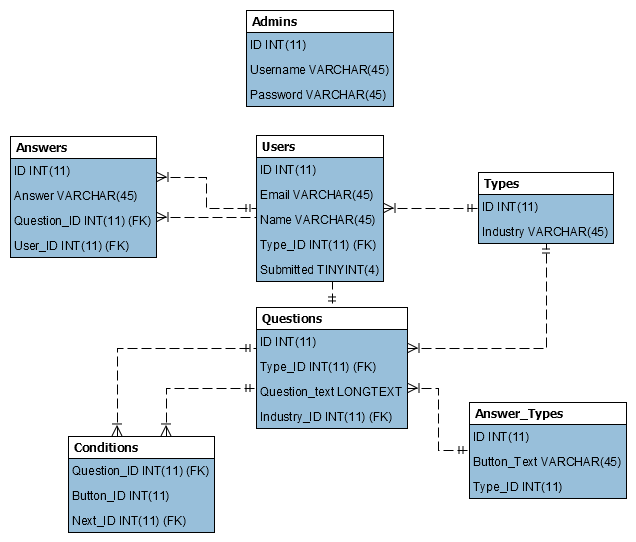
\includegraphics[width=10cm]{ER-diagram.png}
    \caption{ER-diagram över databasen.}
    \label{fig:ER}
\end{figure}

Användbarhetstesterna tillsammans med intervjuandet av försökspersoner resulterade i att de användbarhetskrav gruppen framställt uppfylldes och systemet kunde därmed bekräftas vara tillräckligt intuitivt och uppebart.\\\\
Varje användare loggar in på applikationen med sin emailadress. Detta för att förenkla för svarspersonerna då de skulle slippa att skapa konto och lösenord. Figur \ref{fig:login} visar inloggningssidan för svarspersonerna. Loggan och färgen är hämtad från HCEB:s grafiska profil. \\

\begin{figure}[H]
    \centering
    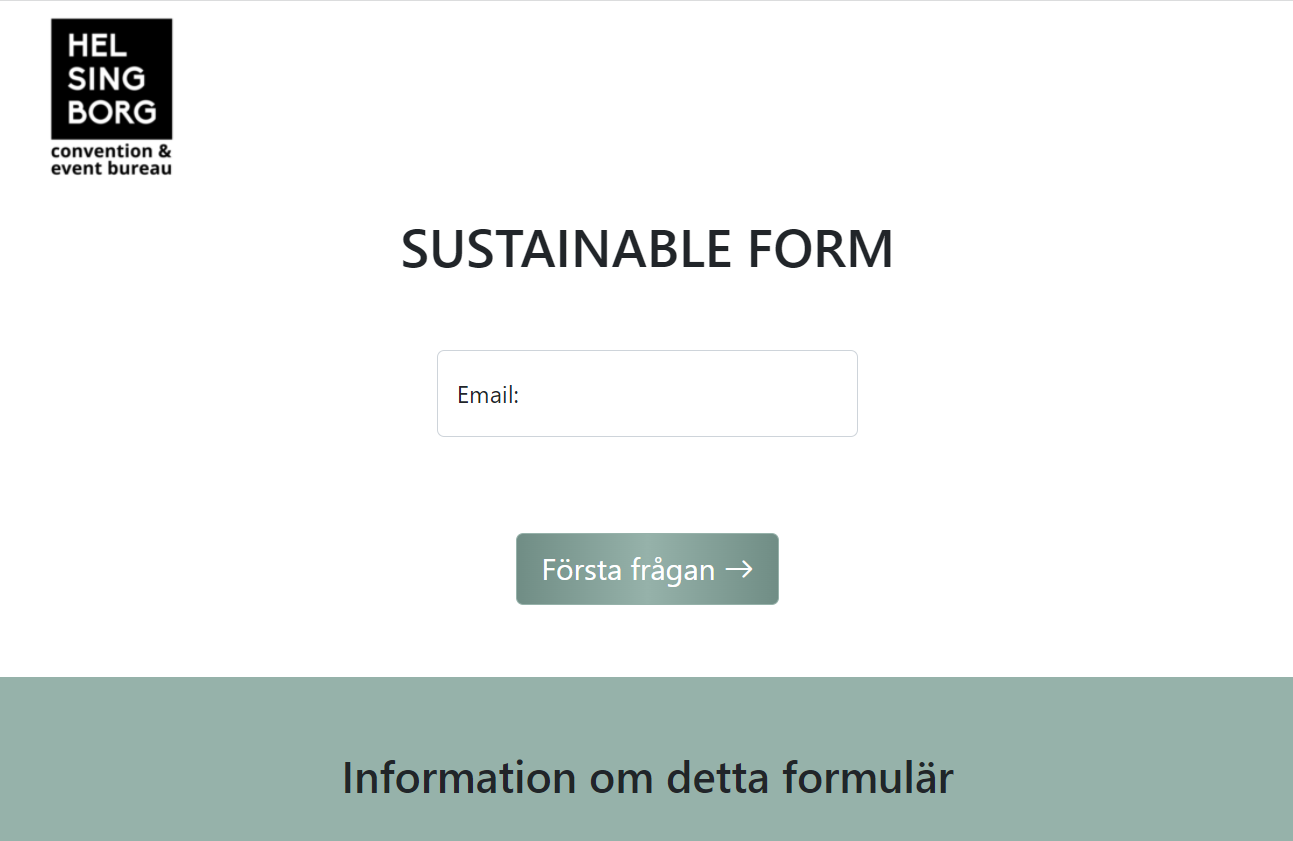
\includegraphics[width=12cm]{log_in_page.png}
    \caption{Inloggningssidan för personer som gör enkäten}
    \label{fig:login}
\end{figure}

Beställaren hade krav på ett enkelt användargränssnitt eftersom svarspersonerna antogs ha varierande teknisk kunskap. Målet var att begränsa antalet valmöjligheter användarna skulle ställas inför. Applikationen kommer att uppfattas som mer intuitiv om användarna slipper undra om de gör rätt eller om en viss länk eller knapp går att klicka på [5]. Därför finns det minimalt med knappar och val i själva formuläret. I databasen har varje företag ett branschattribut knutet till sig. Även här är syftet att begränsa antalet valmöjligheter samtidigt som endast de frågor som faktiskt är riktade till branschen personen företräder visas. I figur \ref{fig:question} nedan syns den inledande frågan för restaurangbranschen.


\begin{figure}[H]
    \centering
    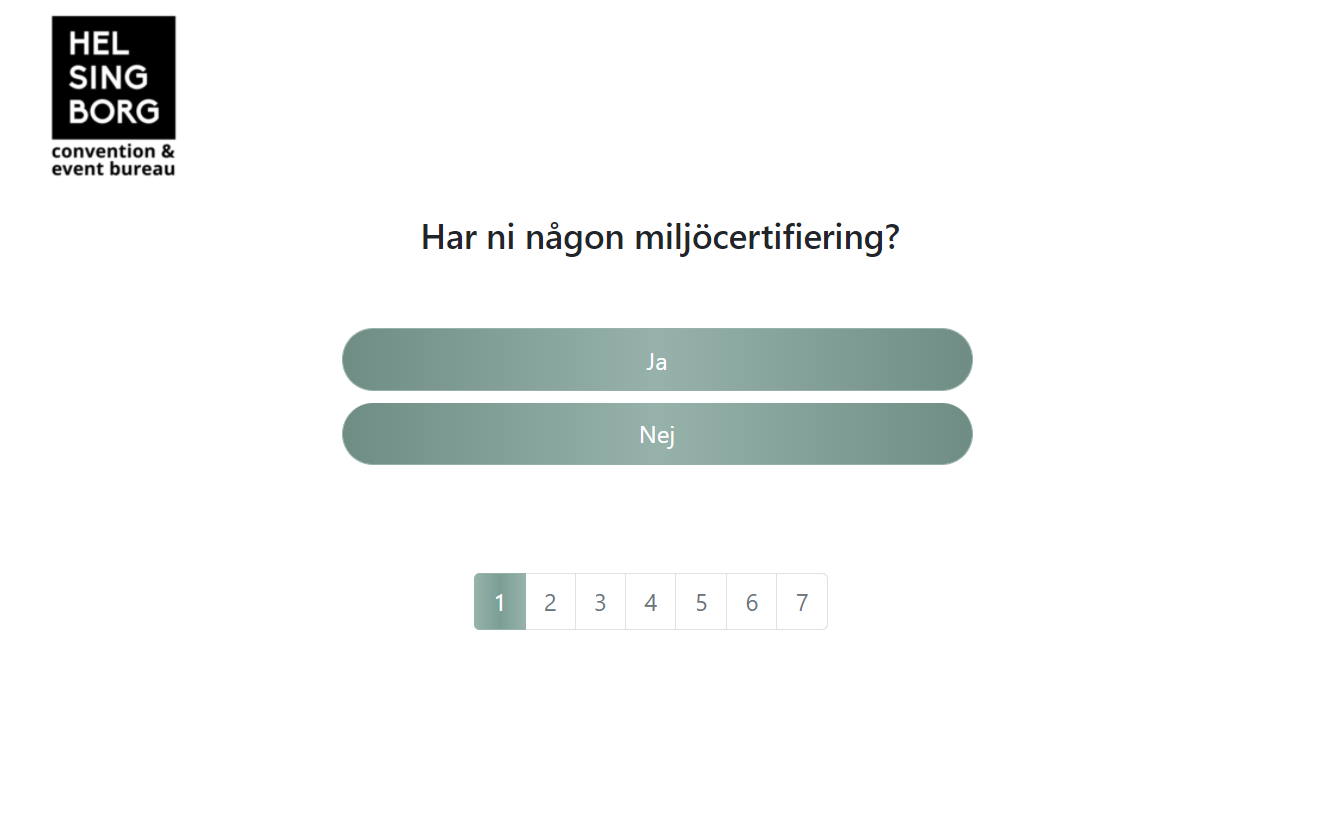
\includegraphics[width=12cm]{question_page.png}
    \caption{Fråga 1 riktad till hotell och restauranger}
    \label{fig:question}
\end{figure}


Samma html-sida användes för samtliga frågor, där själva frågeinnehållet uppdateras dynamiskt med hjälp av JavaScript och Flask när användaren klickar i ett svarsalternativ. Som ett steg i att skapa en mer flexibel och modulär applikation hämtas frågorna och svaren direkt från databasen.

Applikationen innehåller även en administrationssida.
 På adminsidan kan man sammanställa data och få en överblick av statistiken men även söka efter svar från en särskild aktör som man är intresserad av. I figur \ref{fig:admin_login} nedan syns själva inloggningssidan.
 
 \begin{figure}[H]
    \centering
    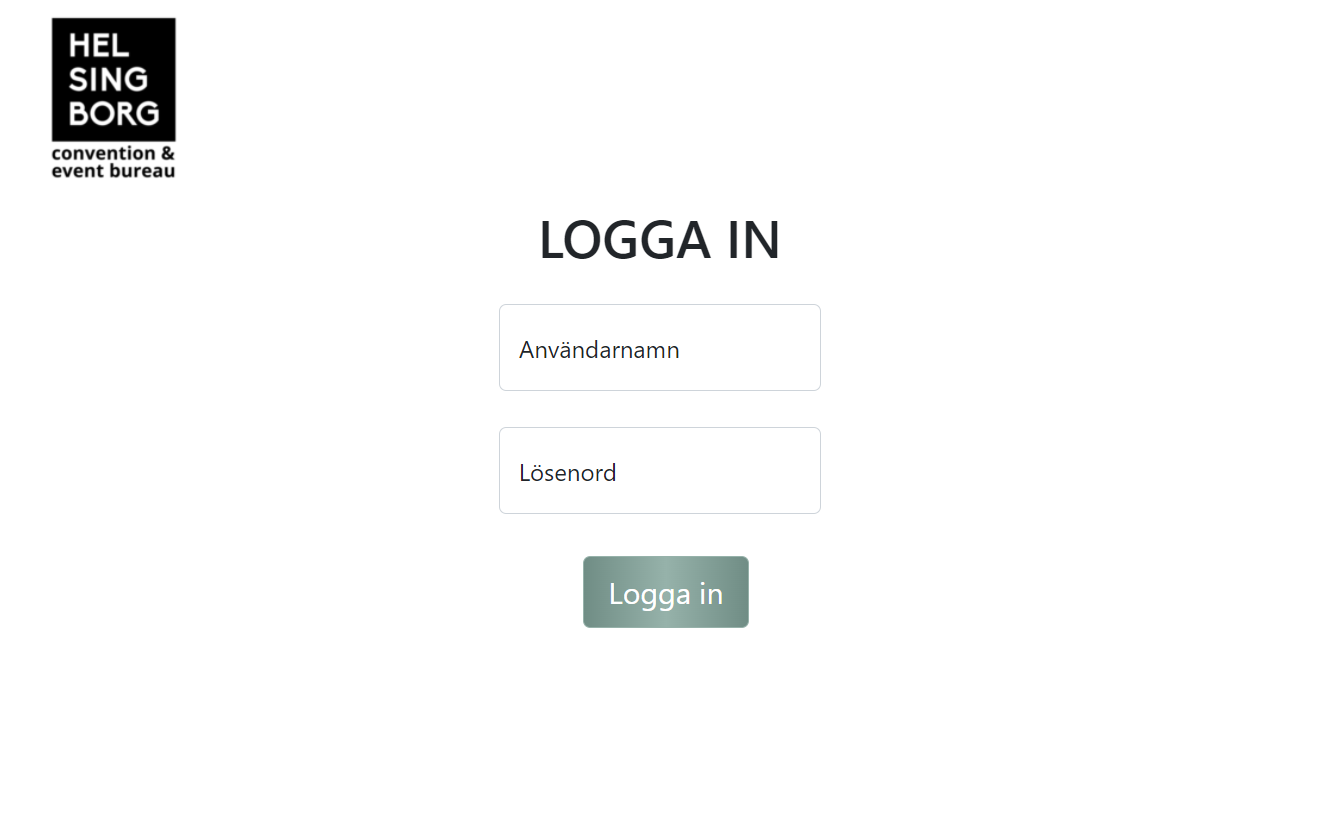
\includegraphics[width=12cm]{admin_log_in.png}
    \caption{Inloggningssida för admin}
    \label{fig:admin_login}
\end{figure}

Adminsidan kan endast nås via URL:en för att inte förvirra personerna som svarar på formuläret. I inloggat läge finns knappvalen "välj bransch", för att se sammanställning av en enskild bransch, "sök rapport", för att se en enskild rapport, och en knapp för att logga ut. Dessutom finns det i högra övre hörnet en kugghjulsikon. När man klickar på den syns en drop-downmeny med val för att byta lösenord och lägga till användare. När admin trycker på någon av dessa kommer en pop-up-ruta med textfält för inmatning av nytt lösen, användare, eller för att söka efter specifik rapport. Figur \ref{fig:admin_index} visar adminsiddan i inloggat läge.

\begin{figure}[H]
    \centering
    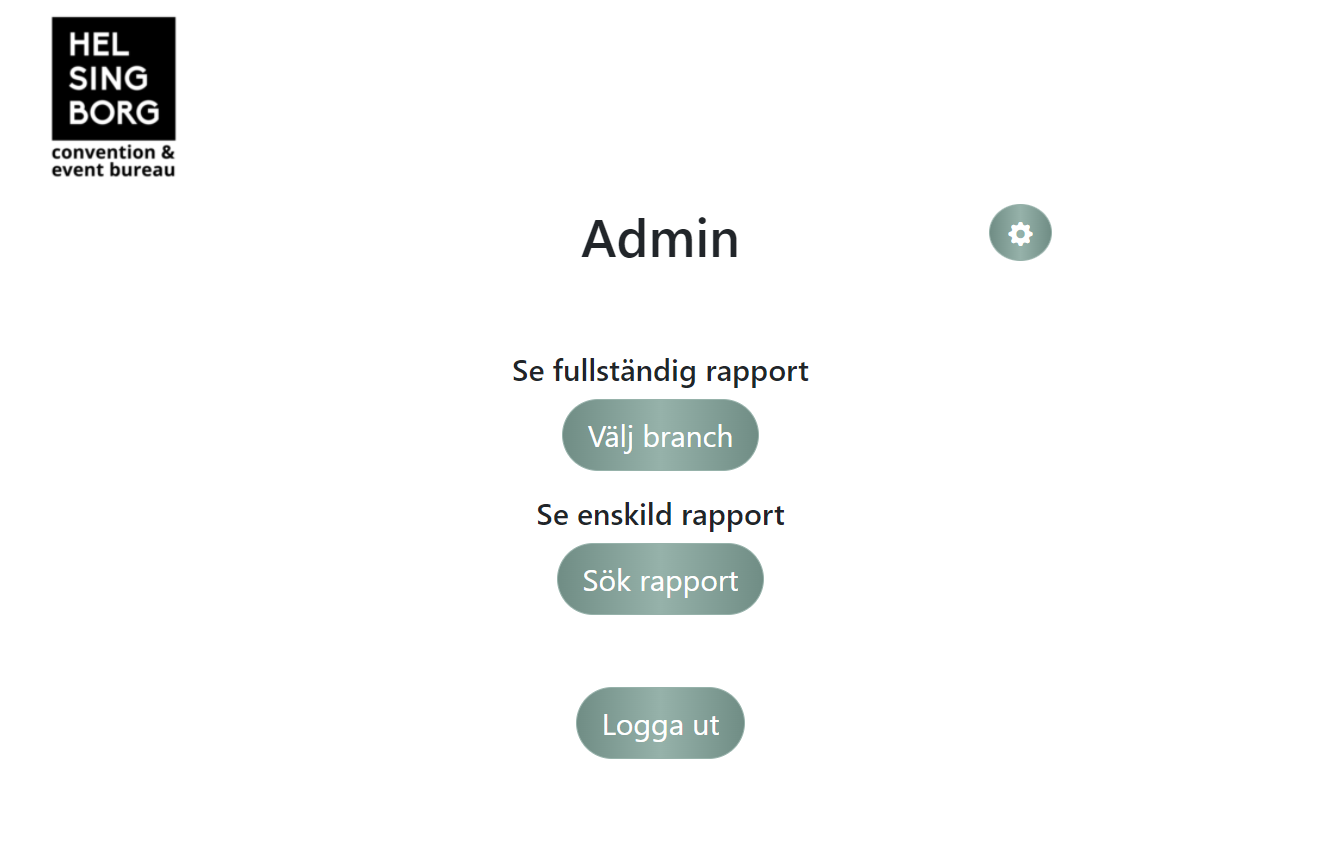
\includegraphics[width=12cm]{admin_index.png}
    \caption{Administrationssidan}
    \label{fig:admin_index}
\end{figure}

Funktionerna som visar inrapporterade data är implementerad med JavaScript och vyn är statisk och har ingen nedladdningsfunktion.
\newpage
\section{Diskussion}
I det här avsnittet förs en kort diskussion om projektets förändrade målbild, rollfördelningen i gruppen och hur väl tidsplaneringen visade sig stämma överrens med verkligheten.
\subsection{Förändrade målbilder}

Projektets mål var inledningsvis att samla in hållbarhetsdata för samtliga fyra områden som ska finnas representerade i GDS-index, vilka förutom besöksnäringen även inkluderade stadens miljöarbete, sociala utveckling och styre. Projektets angränsningsområde har begränsats två gånger under utvecklingens gång. Första gången var under det inledande mötet med beställaren då de klargjorde att det beställda systemet endast skulle fokusera på besöksnäringen - hotell, restaurang, flygplats, högskola och byråer. Andra gången var efter ett uppföljningsmöte med kunden då det meddelade att de samlar in hållbarhetsdata från högskolan och flygplatsen via kontakt över telefon eller mail. Slutprodukten som skulle levereras riktade sig därför enbart mot restauranger, hotell, byråer och evenemangshallar. Även om skalan för projektet ändrades så är resultatet ändå hand i hand med den ursprungliga målbeskrivningen eftersom de absolut flesta aktörer inom besöks- och turistnäringen inom Helsingborgs stad finns inom just dessa tre branscher.


\subsection{Utmaningar under utvecklingen}

\subsubsection{Tekniska utmaningar}
Under projektets gång stötte vi på problem som vi inte hade räknat med från början. Det visade sig vara krångligt att sätta upp databasen med MySQL vid användning av ramverket Flask. Att projektgruppen hade mycket lite erfarenhet av att programmera i Python förenklade inte situationen.\\\\
Ett annat problem som vi stötte på var att kunna skicka POST requests till servern vid implementering av inloggningsfunktionen. Vi hade också problem med att synkronisera vissa funktioner för hemsidan med Flask.\\\\
Den största utmaningen är att driftsätta applikationen, dvs. få upp systemet på en webbserver så att beställaren kan börja använda den.

\subsubsection{Logistiska utmaningar och sjukdom}

När utvecklingen drog igång på allvar hade restriktionerna mot campusförlagd undervisning försvunnit och det fanns en unison vilja att vara fysiskt på plats och arbeta tillsammans som grupp. Redan i ett tidigt stadie märktes det att arbetet fortskred med större hastighet då alla var på plats. I praktiken var det svårt att få till. Hälften av teammedlemmarna är inte bosatta i Helsingborg så oftast var några medlemmar frånvarande på arbetspassen vilket ledde till en mer splittrad utvecklingsprocess och försvårade kunskapsdelning. I riskanalysen utsågs sjukdomsbortfall som en stor risk. Dock blev konsekvenserna av sjukdomsfrånvaro inte lika stora som först befarats. Dock blev konsekvenserna av sjukdomsfrånvaro inte lika stora som först befarats, något som kan bero på att samhällssmittan av Covid-19 var förhållandevis låg under utvecklingen.

\subsection{Rollfördelning och tidsuppskattning}

Gruppen har kompetens inom olika områden och skiftande erfarenhet inom framför allt programmering vilket har lett till att några personer har fått dra ett större lass. Kunskap har delats inom gruppen och det har funnits en vilja att göra så att den som vill förstå implementeringsdetaljer ska kunna få göra det. Projektledarrollen tog Filip sig an på ett bra sätt och var den som samlade gruppen till möten då det ofta var svårt att träffas alla på plats.\\\\
Vår ursprungliga tidsuppskattning för utvecklingsarbetets olika deluppgifter var inte tillräckligt noggrannt planerad. Det fanns inget tydligt mål för hur mycket tid varje teammedlem skulle lägga per sprint och därför kunde ibland vissa uppgifter antingen bli klara mycket fortare än beräknat eller ta ännu längre tid. Dessutom togs det ingen höjd för den tvåveckorsperiod av tentaplugg och tentaskrivning. Det ledde till att vi hamnade efter i planeringen och fick därför lägga mer tid för att ligga i fas igen för att undvika förseningar. Genom att blicka tillbaka tänker vi oss att det har varit en lärande process som belyst vikten av noggrann planering och att försöka göra mer realistiska tidsuppskattningar. \\\\
Backloggen utnyttjades mestadels för tekniska utvecklingen och har främjat arbetsflödet. Det gav en överblick över utförda jobb och så att vi försökte att hålla deadlines.\\\
\section{Råd till studenter för kommande år}

Våra fem råd till studenter som ska läsa kursen kommande året hade varit nedanstående:
\begin{enumerate}

\item  Kommunikationen mellan projektmedlemmarna är viktigt och underlättar arbetet enormt. Om något känns oklart var inte rädda för att ställa frågor för en bättre förståelse. Ha som utgångspunkt att syftet med projektprocessen är att lära sig för att längs vägen nå ett slutmål där alla inom gruppen vill lyckas.
\item Prata tidigt om varandras kompetenser och styrkor för att utnyttja dessa i projektet på bästa sätt. Ta hjälp av varandra och våga utmana er själva för att utvecklas inom något. 
\item  Planera tidigt att jobba tillsammans och inför schemalagda arbetspass där alla kan vara med för att jobba parallellt på olika deluppgifter. På det sättet kan alla bidra med något och arbetet rullas kontinuerligt framåt och det besparas mycket tid. 
\item  Avsätt mycket tid för databasen och integrationen med utvecklingsmiljö. 
\item  Sätt upp tydliga grund rules och ta nödvändiga åtgärder om det skulle behövas.        
\end{enumerate}

\section{Slutsatser}
Brief conclusion: What did you accomplish? What made you succeed or not? 

Projektgruppen lyckades bygga en fungerande rapporteringsverktyg som tillåter användare skicka in hållbarhetsdata utifrån kunden funktionalitetskrav. En sammanställning av hållbarhetsdata kunde göras för att få statistik av en administratör från adminsidan på rapporteringsverktyget. Projektgruppen har tillämpat och lärt sig använda det agila arbetssättet samtidigt som vi har utifrån kundens uppdrag hjälpt till att utveckla ett  rapporteringsverktyg som kan användas till ett gott syfte för stadens hållbarhetsutveckling. Arbetet var utmanade men samtidigt väldigt lärorikt och kul. 

\section{Referenser}
[1] Sharp. H, Preece, J., \& Rogers, Y. (2019). \textit{Interaction Design - Beyond Human/Computer Interaction}. John Wiley \& Sons. Hoboken, New Jersey, United States. \\

\noindent
[2] Kniberg \& H. Skarin, M. (2010), Kanban And Scrum Making Most of Both, C4Media Inc., U.S. \\\\
\noindent
[3] Matz, K. (2013). Designing Usable Apps, An Agile Approach to User Experience Design. Hämtad 2021-
10–10 från https://canvas.education.lu.se/courses/13397/files/
1703747?wrap=1 \\\\
\noindent
[4] Eriksson, M. \& Lilliesköld J. (2005), Handbok f̈or mindre projekt, Liber, Solna, Sweden, pp. 42–46. \\\\

\noindent
[5] Krug S., (2010). Don’t Make Me Think, New Riders Publishing, Indianapolis, IN, United States. \\\\


\bibliographystyle{alpha}


\end{document}
